\section{Introduction to Interactive Proofs}

The standard idea of a mathematical proof is intuitively provided by the complexity class $\np$, which is the set of problems that can be efficiently verified by a polynomial-time verifier (a Turing Machine) given a polynomial time \textit{witness}. Fundamentally, this witness is nothing but a proof of a statement. We recall the formal definition of the class $\np$.

\begin{definition}[$\np.$]
	A language $L$ is in $\np$ iff there exists a polynomial-time verifier $M$ and a polynomial $p$ such that
	\begin{align}
		\forall x\in L, \exists w:|w|=p(|x|)&\implies M(x, w)=1\\
		\forall x\notin L, \forall w:|w|=p(|x|)&\implies M(x,w)=0
	\end{align}
\end{definition}

Here, the first predicate $(1)$ may be termed \textit{completeness}, since it certifies that a proof exists for all instances of $L$, and the second predicate $(2)$ may be termed \textit{soundness}, since it certifies that no proof exists for any $x\notin L$.

The interesting idea here is that $\np$ can be taken to be a proof system between a (potentially computationally unbounded) prover and an efficient verifier.

\begin{figure}[h]
	\centering
	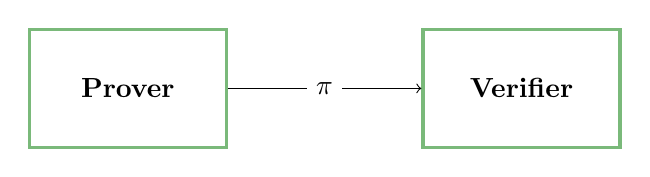
\begin{tikzpicture}[
		squarenode/.style={rectangle, draw=ForestGreen!60, very thick, minimum height=15mm, minimum width=25mm}]
		
		\node[squarenode] (prover) at (0,0) {\textbf{Prover}};
		\node[squarenode] (verifier) at (5, 0) {\textbf{Verifier}};
		
		\draw [->] (prover) -- (verifier) node [midway, fill=white] {$\pi$};
	\end{tikzpicture}
	
	\caption{$\np$ as a proof system.}
\end{figure}

\subsection{Interactive Proofs}
The idea of interactive proofs was originally formalized by Goldwasser, Micali, and Rackoff \cite{10.1145/22145.22178} in 1985. The key insight into this definition is that $\np$ can be equipped with two additional tools to make it more powerful, which leads to a new and groundbreaking form of computation.

\textbf{Remark.} We will denote the prover by $\prover$ and the verifier by $\verifier$.

\begin{enumerate}
	\item\textbf{Interaction.} Instead of a single prover message (consisting of the proof) from $\prover$ to $\verifier$, $\verifier$ is also allowed to communicate messages to the prover, and multiple rounds of communication are allowed.
	\item\textbf{Randomness.} The verifier is allowed access to a random string. 
\end{enumerate}

We formally define interactive proofs as follows.

\begin{definition}[Interactive Proofs.]
	An interactive proof for $L$ is a pair $(\prover,\verifier)$ such that the following are satisfied:
	\begin{align*}
		\forall x\in L, &\Pr[\langle\prover(x), \verifier(x, \cdot)\rangle=1]=1\\
		\forall x\notin L,\forall\tilde{\prover} &\Pr[\langle\tilde{\prover}(x), \verifier(x, \cdot)\rangle=1]\leq\frac{1}{2}
	\end{align*}
	Here, $\langle\prover(x), \verifier(x, \cdot)\rangle$ is the output of the interaction between $\prover$ and $\verifier$. The soundness error need not be $1/2$ and any large gap suffices.
\end{definition}

The complexity class of languages which have an interactive proof is termed $\ip$.

\subsection{IP for Graph Non-Isomorphism}

We know that $\np\subseteq\ip$. Is the other way around true? In other words, do interaction and randomness give additional power to the proof system? We now see an example of a non-trivial IP for a problem not known to be in $\np$.

\paragraph{Graph Non-Isomorphism} The problem of checking whether two graphs $G_1$ and $G_2$ are isomorphic (ie. whether there is a suitable permutation of the vertices of $G_1$ such it equals $G_2$) is in $\np$, since the permutation is a polynomial-size witness. GI is one of the problems known to be in $\np$ that, as far as we know, has not yet proven to be $\np$-complete. GNI (graph non-isomorphism) is the problem of determining whether $G_1$ and $G_2$ are \textit{not} isomorphic, which is clearly in $co\np$, but it is still unknown whether it is $co\np$-complete.

In the following protocol, both have access to both graphs, but the verifier does not have the computational power to check non-isomorphism.

\begin{figure}[h]
	\begin{mdframed}[
		linecolor=black,
		linewidth=1pt,
		roundcorner=5pt,
		backgroundcolor=white,
		userdefinedwidth=\textwidth,
		]
		\vspace{2mm}
		\begin{enumerate}
			\item $\verifier$ samples a random bit $b\leftarrow\{0,1\}$.
			\item $\verifier$ permutes the vertices of graph $G_b$ randomly and sends the permuted graph $G'$ to $\prover$.
			\item If $G_1\not\cong G_2$, then $\prover$ sends $G''=G_b$ to $\verifier$.
			\item Otherwise, $\prover$ sends a random $G''\leftarrow\{G_1, G_2\}$ to $\verifier$.
			\item If $G''=G_b$, the verifier outputs $1$. Otherwise it outputs $0$.
		\end{enumerate}
		\vspace{2mm}
	\end{mdframed}
	\caption{IP for Graph Non-isomorphism.}
	\label{fig:2}
\end{figure}

\textbf{Analysis.} First, it is clear that $\prover$ will only be able to send $G_b$ back with $100\%$ certainty if $G_1\not\cong G_2$. Otherwise, it won't be able to uniquely determine which graph was permuted by $\verifier$.

We now formally show that the above protocol is an interactive proof for $\mathsf{GNI}$ by verifying completeness and soundness.

\vspace{3mm}

\begin{theorem}
	The protocol in \ref{fig:2} is an interactive proof for $\mathsf{GNI}$.
\end{theorem}

\begin{proof}
	\textbf{Completeness.} If $(G_1, G_2)\in\mathsf{GNI}$, then an honest prover will always be able to correctly find $G_b$ by running an isomorphism check on both graphs. Thus, $\Pr[\langle\prover(x), \verifier(x, \cdot)\rangle=1]=1$.
	
	\textbf{Soundness.} If $(G_1, G_2)\notin\mathsf{GNI}$, then a dishonest prover cannot do better than randomly guessing some $G''$ and sending it. In this case, $\Pr[\langle\prover(x), \verifier(x, \cdot)\rangle=1]=\frac{1}{2}$, because it will output the correct $G_b$ with probability $1/2$.
\end{proof}

\vspace{2mm}

A natural question is that if $\prover$ is so powerful, why can't it simply \textit{simulate} $\verifier$ and determine what bit $\verifier$ has picked? The answer is that $\verifier$ has access to \textit{private randomness} that $\prover$ does not have access to. This is a crucial part of the protocol \textbf{--} if the prover had access to this randomness, the protocol fails, since even in the case of isomorphism, a dishonest prover would be able to determine which graph the $\verifier$ chose.

It turns out that private randomness is not necessary for $\ip$. We will later see how proofs for all languages can be turned into public-coin proofs where $\prover$ can convince $\verifier$ without $\verifier$ having any additional information that $\prover$ does not.

\subsection{$\ip=\pspace$}

We now show the first part of a classical result that upper bounds the class $\ip$. The full result was first shown by Adi Shamir \cite{10.1145/146585.146609} in 1990 and formally published in 1992. We thus have good reason to believe that interactive proofs form a much broader class of computation than $\np$, and that randomness and interactivity both give additional amount of power to a proof system.

\begin{theorem}
	\label{thm:ipsubsetpspace}
	$\ip\subseteq\pspace$.
\end{theorem}

\begin{proof}
	Let $L\in\ip$, and let $(\prover,\verifier)$ be an IP for $L$. We show that $L\in\pspace$. First, we fix an instance $x$, and define
	$$\mathbf{q}_x=\max_{\tilde{\prover}}\Pr_{r}[\langle\tilde{\prover}(x), \verifier(x, \cdot)\rangle=1].$$
	Concretely, $\mathbf{q}_x$ is the maximum probability of acceptance over all possible provers. It is clear that $\mathbf{q}_x=1$ if $x\in L$ and $\leq 1/2$ otherwise. Thus if we manage to calculate $\mathbf{q}_x$ in polynomial space, we are done. The difficulty here is simulating all provers, since the prover can be a machine of potentially unbounded complexity.
	
	Instead of attempting to simulate the prover, we will attempt to simulate the set of all possible transcripts (which must be polysize), and in the process simulate the \textit{optimal prover strategy}. Let a partial transcript be $\pi_i=(a_1,b_1, a_2,b_2,\dots a_i,b_i)$, where the $a_i$ are the prover's messages and the $b_i$ are the verifier's.
	
	\textbf{Definition.} Let $P^{*}(x, \pi_i)$ be a function that outputs $a_{i+1}^{*}$, the prover message that maximizes probability of $\verifier$ accepting.
	
	\textbf{Lemma.} $P^{*}\in\pspace\implies\mathbf{q}_x\in\pspace$.
	
	\textit{Proof.} Let $d(x,r)$ be the decision of $\verifier$ when it interacts with $P^{*}$. Then $\mathbf{q}_x$ can be written as
	$$\frac{\sum_{r\in\mathcal{R}}d(x,r)}{|\mathcal{R}|}$$
	Each $d(x,r)$ can be calculated using $P^{*}$. In particular, we take $P^{*}(x,\bot)=a_{1}^{*}, \verifier(x, a_1^{*})=b_1,\dots$, till we get the verifier's output. Here we are simulating the verifier in polytime, and since $P^{*}\in\pspace$, the total computation occurs in $\pspace$. Once we have found each $d(x,r)$, we can simply add and calculate the average, since $\mathcal{R}$ is only polynomial in size.\qed
	
	Our problem now reduces to showing that $P^{*}$, the optimal prover strategy, is in $\pspace$. This requires some amount of backward induction over the inputs, but the heuristic is as follows. If the protocol for $L$ is $k$-round, then if we have the optimal $k-1$ messages, finding the optimal $k^{\text{th}}$ message is as simple as iterating over all the possible polynomial-length output messages, running the verifier over each one (with different randomness) and choosing the one which maximizes verifier acceptance over the largest amount of random strings. If we have access to $k-2$ messages, we can do this recursively. We induct all the way back to the case in which we have no messages. $k$ is constant, so we can be assured that that total amount of space used is polynomial. Simulating the verifier again requires polynomial space. All other considerations such as keeping a counter can be done in polynomial space or less. 
	
	Thus we can calculate $\mathbf{q}_x$ in polyspace. The value of $\mathbf{q}_x$ determines whether $x\in L$ or not. We are done.
\end{proof}
